\documentclass[conference]{IEEEtran}
\usepackage[T1]{fontenc}
\usepackage{amsmath,amssymb,amsthm}
\usepackage{graphicx}
\usepackage{booktabs}
\usepackage{tikz}
\usetikzlibrary{arrows.meta,positioning,fit}
\usepackage[hidelinks]{hyperref}
\newtheorem{theorem}{Theorem}
\newtheorem{lemma}{Lemma}
\newtheorem{proposition}{Proposition}

\begin{document}

\title{TRIAD-BISR: On-Chip Exact Allocation of Spare Words, Partition-Steered Spare Columns and an ECC Budget for an Embedded SRAM Macro}

% Fill in before submission.
\author{\IEEEauthorblockN{Author names to be added}
\IEEEauthorblockA{Affiliation to be added\\e-mail to be added}}

\maketitle

\begin{abstract}
Embedded memories are repaired with spare rows and columns, and many of them also carry an
error-correcting code (ECC) for soft errors. Letting the ECC absorb hard faults raises yield but
removes the soft-error protection of every word that relies on it. We study the repair problem in
which spare words, spare columns and ECC are allocated together and the number of ECC-reliant words is
capped by a programmable budget $K$. We show that the problem stays NP-complete for every fixed $K$,
give must-repair rules and a tight bound of $R+S(R+K)+K$ faulty words on the fault store, and show that
for a fixed number of spare columns it is solved exactly by enumeration. We build this into a
self-test and self-repair wrapper around an unmodified OpenRAM macro in SkyWater 130\,nm, in which each
spare column is steered to a different bit in each address partition by a small table. On 10\,000
random fault maps per point, with two spare words and two spare columns, the defect count tolerated at
a 90\,\% repair rate rises from 3.2 for exact two-dimensional repair to 9.3 with 16 partitions and
$K=8$ under a mixed defect model, and the 90\,\% point does not move when line defects dominate. Each ECC-reliant word
adds 0.0145 FIT of detected uncorrectable errors under an assumed 1000 FIT/Mbit. The wrapper is taken
from RTL to GDS with open-source tools; routing, LVS, timing and the design-rule check of the final GDS
pass, while one antenna violation and maximum-slew and fanout violations remain open.
\end{abstract}

\begin{IEEEkeywords}
memory built-in self-test, built-in redundancy analysis, built-in self-repair, error-correcting code,
spare allocation, OpenRAM, SkyWater 130\,nm
\end{IEEEkeywords}

\section{Introduction}
Memory built-in self-test (MBIST) finds faulty cells, built-in redundancy analysis (BIRA) decides
which spare elements replace them, and built-in self-repair (BISR) applies the decision
\cite{huang2003,kawagoe2000}. Choosing spare rows and columns is NP-complete \cite{kuo1987}, so
on-chip analysers are usually heuristics. Separately, a single-error-correcting, double-error-detecting
(SEC-DED) code \cite{hsiao1970} can hide a hard fault, and several schemes use it for repair
\cite{lu2016,sun2011,lv2021,han2021}. The cost is reliability: a word that spends its correction on a
hard fault has none left for a soft error.

Neither idea is new, and we claim neither. Lv \emph{et al.} give an optimal repair analysis for
memories with in-memory ECC, run on the tester \cite{lv2021}; Han \emph{et al.} reduce ECC use in a
tester-side pattern-matching analysis \cite{han2021}; EBISR applies ECC first and spares to what is
left, on chip \cite{lu2016}; Sun \emph{et al.} describe a BIRA that exploits on-chip ECC
\cite{sun2011}. Steering a spare column to different bits in different row partitions was proposed by
Rab, Bawa and Touba inside the array with fuses \cite{rab2009}. Wrapper-level repair of macros without
spares exists in commercial tools and in the open-source autoMBIST generator \cite{automb}. These
statements rest on the literature we surveyed; the full texts of \cite{lv2021,lu2016,han2021} were not
available to us, so we do not claim that no earlier work overlaps with ours.

What we add is the combination, implemented and measured:
\begin{itemize}
\item a formulation in which ECC is a third repair resource with a programmable cap $K$ on
ECC-reliant words, with hardness, must-repair rules, a tight fault-store bound and a polynomial case
(Section~\ref{sec:theory});
\item an on-chip allocator that is exact for this model, with spare columns steered per address
partition from a table in the wrapper of an unmodified macro (Section~\ref{sec:arch});
\item an evaluation on identical fault maps against exact two-dimensional repair, ECC-first schemes
and the on-chip analysers of autoMBIST, with the reliability cost in FIT (Section~\ref{sec:eval});
\item an open RTL-to-GDS implementation in SkyWater 130\,nm with its sign-off status reported as it
is (Section~\ref{sec:impl}).
\end{itemize}

\section{Budgeted Tri-Resource Repair}\label{sec:theory}
A fault map is a bipartite graph $G=(A,B,F)$ of words $A$ and bit columns $B$; $(w,c)\in F$ if bit $c$
of word $w$ is faulty. Given $R$, $S$ and $K$, a \emph{repair} is a set $X\subseteq A$, $|X|\le R$, of
words replaced by spare words and a set $Y\subseteq B$, $|Y|\le S$, of replaced columns such that
(i) every word outside $X$ has at most one faulty bit outside $Y$, and (ii) the number $E$ of words
outside $X$ with exactly one such bit is at most $K$. Condition (i) is what SEC-DED can absorb;
(ii) is the ECC budget. With $K=0$ this is constrained bipartite vertex cover \cite{kuo1987,fernau2001,chen2003}.

\begin{theorem}\label{th:np}
The problem is NP-complete for every fixed $K\ge 0$, for unbounded $K$, and for unbounded $K$ with
$R=0$.
\end{theorem}
\emph{Sketch.} For fixed $K\ge1$, pad an instance of the $K=0$ problem with $K$ new words, each with
one fault in a private column; a repair that spends spares on $t$ gadgets leaves at most $t$ words of
$G$ on ECC, and the $t$ spares can be moved onto them. For unbounded $K$, give every word a pendant
fault in a private column. For $R=0$, encode a graph by one column per vertex and one two-fault word
per edge; a repair is a vertex cover. \hfill$\square$

So ECC does not make allocation easy, even without spare words.

\begin{lemma}[Must-repair]\label{lem:mr}
With $R'$ and $S'$ spares still free, a column with more than $R'+K$ faulty words is in every repair,
and so is a word with more than $S'+\epsilon$ faulty bits, where $\epsilon=1$ if $K\ge1$ and $0$
otherwise.
\end{lemma}

\begin{theorem}[Fault-store bound]\label{th:kernel}
After applying Lemma~\ref{lem:mr} to a fixed point and deleting covered faults, a repairable
instance has at most $R+S(R+K)+K$ faulty words, and the bound is attained.
\end{theorem}
\emph{Proof.} In a repair of the reduced instance a faulty word is in $X$ (at most $R$ words), has a
fault in a column of $Y$ (each such column is not must-repair, so at most $R+K$ words per column), or
has a single fault outside $Y$ and is counted in $E$ (at most $K$). \hfill$\square$

A store of this size therefore overflows only on unrepairable memories. For $K=0$ the bound is the
word-count form of the classical kernel, which is essentially optimal \cite{jansen2016}.

\begin{theorem}[Exact search]\label{th:search}
Branching on a word with two remaining faults $b_1,b_2$ into ``replace the word'', ``replace column
$b_1$'' and ``replace column $b_2$'', and, when no such word is left, spending the remaining spares in
order of decreasing gain, returns a repair with minimum $E$ after at most $3^{R+S}$ leaves.
\end{theorem}

\begin{theorem}[Fixed $S$]\label{th:enum}
For a fixed number $S$ of spare columns the problem is solved in $O(W^S|F|)$ time for words of $W$
bits: for every $Y$ with $|Y|\le S$, every word with two or more remaining faults must take a spare
word, and the spare words left over go to single-fault words.
\end{theorem}

For $W=30$ and $S=2$ there are 466 column sets. Theorem~\ref{th:np} shows that the exponent cannot be
removed in general.

\emph{Partitions.} Let the words be split into $P$ partitions by their upper address bits, and let
each spare column replace a possibly different bit in each partition.

\begin{proposition}\label{prop:dp}
Let $e_p(r)$ be the minimum $E$ of partition $p$ alone with $r$ spare words. The partitioned instance
is repairable iff there are $r_p$ with $\sum_p r_p\le R$ and $\sum_p e_p(r_p)\le K$; the optimum is
found by a dynamic programme over the partitions.
\end{proposition}
Faults in different partitions share neither words nor column choices, so only $R$ and $K$ couple
them.

A greedy allocator is not exact: with $R=0$, $S=1$, $K=2$ and three words with faulty bits $\{0\}$,
$\{2\}$ and $\{1,2\}$, repair-most leaves three ECC words while replacing column 2 leaves two. All
statements above are exercised by tests against exhaustive search on small instances; the proofs have
not been reviewed independently.

\section{Architecture}\label{sec:arch}
\begin{figure}[t]
\centering
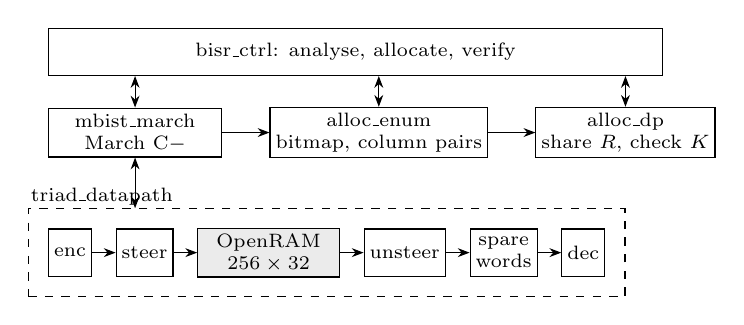
\begin{tikzpicture}[font=\scriptsize, node distance=3mm and 3mm,
  b/.style={draw, minimum height=6mm, inner sep=2pt, align=center}, >={Stealth[length=1.5mm]}]
\node[b, minimum width=78mm] (ctrl) {bisr\_ctrl: analyse, allocate, verify};
\node[b, below=4mm of ctrl.south west, anchor=north west, minimum width=22mm] (march) {mbist\_march\\March C$-$};
\node[b, right=6mm of march, minimum width=22mm] (enum) {alloc\_enum\\bitmap, column pairs};
\node[b, right=6mm of enum, minimum width=22mm] (dp) {alloc\_dp\\share $R$, check $K$};
\draw[->] (march) -- (enum); \draw[->] (enum) -- (dp);
\draw[<->] (march.north) -- (march.north |- ctrl.south);
\draw[<->] (enum.north) -- (enum.north |- ctrl.south);
\draw[<->] (dp.north) -- (dp.north |- ctrl.south);
\node[b, below=9mm of march.south west, anchor=north west] (enc) {enc};
\node[b, right=of enc] (st) {steer};
\node[b, right=of st, fill=black!8, minimum width=18mm] (ram) {OpenRAM\\$256\times32$};
\node[b, right=of ram] (ust) {unsteer};
\node[b, right=of ust] (sw) {spare\\words};
\node[b, right=of sw] (dec) {dec};
\draw[->] (enc)--(st); \draw[->] (st)--(ram); \draw[->] (ram)--(ust); \draw[->] (ust)--(sw); \draw[->] (sw)--(dec);
\node[draw, dashed, fit=(enc)(dec), inner sep=2.5mm, label={[anchor=south west, inner sep=1pt]north west:triad\_datapath}] (dpth) {};
\draw[<->] (march.south) -- (march.south |- dpth.north);
\end{tikzpicture}
\caption{Self-test and self-repair wrapper around the macro. Steering table, spare words and the
signature chain are registers of the datapath.}
\label{fig:arch}
\end{figure}

The memory is the OpenRAM macro \texttt{sky130\_sram\_1kbyte\_1rw1r\_32x256\_8}
\cite{guthaus2016,cirimelli2023}, used unchanged. Of its 32 bits per word, bits 0--29 hold a Hsiao
(30,\,24) codeword and bits 30--31 are the two spare columns. The $R=2$ spare words are flip-flop
registers in the wrapper, selected by address comparison (Fig.~\ref{fig:arch}).

\emph{Datapath.} The 256 words form $P=16$ partitions of 16 words. For each partition a steering
table holds, for each spare column, a valid bit and the code bit it replaces. A write encodes the
data, copies the two named code bits into the spare columns and writes 32 bits. A read puts the spare
columns back in place, substitutes a spare word when the address matches, and decodes. The macro
launches its output on the falling clock edge, so these steps share half a cycle.

\emph{Allocation.} Because $S=2$, the hardware uses Theorem~\ref{th:enum} per partition and
Proposition~\ref{prop:dp} across partitions; it needs neither a content-addressable fault store nor a
search stack. The fault store is the $16\times32$ bitmap of one partition and cannot overflow. In the
first pass, for each partition, March C$-$ \cite{vandegoor1993} runs on the raw 32 bits with six data
backgrounds, the enumerator tries the column pairs among the columns that have faults, and for each
it counts words with two or more remaining faults and words with one. A fault in a spare column is
moved to the bit it would replace, so a bad spare cell is never chosen where it is needed. The result
is $e_p(q)$ for $q=0,\dots,R$, and the dynamic programme is updated. The memory is repairable if the
optimum does not exceed $K$. The second pass revisits the partitions, programs the steering table and
assigns spare words. The third pass runs March C$-$ on the whole memory through the repaired datapath
with ECC; a mismatch or an uncorrectable error fails the repair.

\emph{Repair signature.} The process has no eFuse, so the repair is soft. The steering table and the
spare-word addresses form a 210-bit shift chain that is exported after the test and reloaded after
reset.

\emph{Limits of the scheme.} Partitions are tested one at a time, so coupling faults between
partitions and address-decoder faults appear only in the third pass, which reports failure rather
than re-analysing. Spare words are assumed fault-free. The hardware minimises $E$ and then the number
of spare words.

\section{Evaluation}\label{sec:eval}
\subsection{Repair rate}
All allocators receive the same fault maps: 10\,000 per point for 1 to 30 defects on a
$256\times30$-bit array with a column multiplexing factor of two, $S=2$ and fault-free spares. Defects
are single cells, horizontal or vertical pairs, $2\times2$ clusters, word lines and bit lines, drawn
from four mixes: \emph{date06} (40\,\% cells, 40\,\% pairs, 20\,\% clusters), \emph{kang-dl} (80\,\%
cells, 10\,\% rows, 10\,\% columns), \emph{kang-dh} (45/28/27) and our own \emph{mixed} set (70\,\% cells,
14\,\% pairs, 6\,\% clusters, 5\,\% rows, 5\,\% columns). The first three follow mixes reported in the
repair-analysis literature as collected by a literature search; we have not checked them against the
original papers.

\begin{table}[t]
\caption{Defects per memory tolerated at a 90\,\% repair rate ($R=2$, $S=2$)}
\label{tab:n90}
\centering
\begin{tabular}{@{}llrrrrr@{}}
\toprule
Mix & $K$ & P16 & P4 & P1 & EF+BB & 2-D \\
\midrule
date06 & 0 & 8.3 & 4.4 & 2.5 & 2.5 & 2.5 \\
date06 & 8 & 21.5 & 11.5 & 7.0 & 7.0 & 2.5 \\
mixed & 0 & 5.5 & 4.4 & 3.2 & 3.1 & 3.2 \\
mixed & 8 & 9.3 & 9.2 & 8.2 & 5.4 & 3.2 \\
kang-dl & 0 & 4.4 & 4.1 & 3.3 & 3.3 & 3.3 \\
kang-dl & 8 & 5.4 & 5.4 & 5.4 & 4.3 & 3.3 \\
kang-dh & 0 & 2.2 & 2.2 & 2.2 & 2.2 & 2.2 \\
kang-dh & 8 & 2.2 & 2.2 & 2.2 & 2.2 & 2.2 \\
\bottomrule
\multicolumn{7}{@{}p{0.95\columnwidth}@{}}{\footnotesize P16, P4, P1: this work with 16, 4 and 1
partitions. EF+BB: ECC first with exact 2-D analysis, then spare buy-back. 2-D: exact repair without ECC.}
\end{tabular}
\end{table}

\begin{figure}[t]
\centering
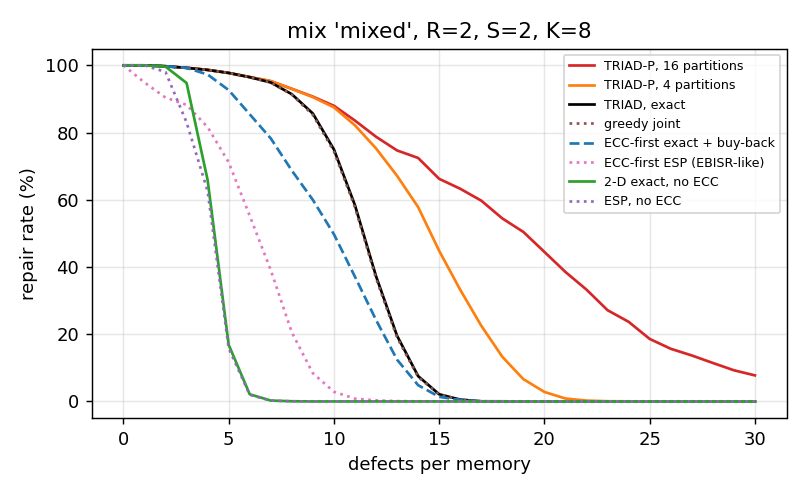
\includegraphics[width=\columnwidth]{../results/protocol/protocol_mixed_R2_S2_K8.png}
\caption{Repair rate against defects per memory, mixed defects, $R=2$, $S=2$, $K=8$.}
\label{fig:rr}
\end{figure}

Table~\ref{tab:n90} and Fig.~\ref{fig:rr} show three things. Partitioned steering helps most when
cells and clusters dominate (date06: 2.5 to 8.3 at $K=0$) and not at all when lines dominate
(kang-dh, at the 90\,\% point), where the spare words are the limit. An ECC budget raises the tolerance for cell defects
(date06, one partition: 2.5 to 7.0 with $K=8$). With $K=0$ and one partition the allocator coincides
with exact 2-D repair, as it must. An exact search buys little over a greedy allocator of the same
formulation (at most 0.4 points of yield in an earlier study on the same array); the gain comes from
the formulation, and allocating jointly outperforms ECC-first with buy-back when lines are present
(mixed, $K=8$: 8.2 against 5.4).

On a $4096\times39$ array with $R=8$, the mixed set and 1\,000 maps per point, the picture is the
same: at $S=2$, $K=0$ the tolerated count is 3.1 for exact 2-D repair and 7.5 with 64 partitions; at
$K=8$ it is 9.0 without partitions and 10.2 with 16.

\subsection{Comparison with autoMBIST}
autoMBIST \cite{automb} solves the 2-D problem exactly on the tester; the analysers it places on the
chip are a one-pass and a two-pass heuristic, documented as approximations, for which it ships a
decision-level Python model. We ran that model unchanged (commit \texttt{032deb05}) on our fault maps
with two spare rows and two spare columns, a spare row replacing one word (Table~\ref{tab:amb}). Its
exact solver and ours agreed on all 800\,000 maps.

\begin{table}[t]
\caption{Repair rate (\%) on identical fault maps, 10\,000 maps per point}
\label{tab:amb}
\centering
\begin{tabular}{@{}lrrrrrr@{}}
\toprule
 & & \multicolumn{3}{c}{autoMBIST} & \multicolumn{2}{c}{this work} \\
\cmidrule(lr){3-5}\cmidrule(l){6-7}
Mix & $n$ & 1-pass & 2-pass & exact & $K{=}8$ & P16, $K{=}8$ \\
\midrule
mixed & 4 & 35.0 & 65.6 & 65.9 & 98.6 & 98.6 \\
mixed & 6 & 0.3 & 2.0 & 2.1 & 96.5 & 96.5 \\
mixed & 8 & 0.0 & 0.1 & 0.1 & 91.4 & 93.0 \\
kang-dl & 4 & 45.6 & 68.9 & 69.6 & 94.9 & 94.9 \\
kang-dl & 6 & 0.3 & 3.5 & 3.7 & 87.8 & 87.8 \\
kang-dh & 4 & 6.1 & 26.2 & 27.6 & 63.3 & 63.3 \\
\bottomrule
\end{tabular}
\end{table}

The two-pass heuristic is close to exact, and the gap to our numbers is the gap between repair with
and without ECC and partitions, which cost six check bits per word and the steering table. In
autoMBIST's native model of a column-multiplexed macro a spare row replaces a physical row of two
words, which helps it for line defects (kang-dh, four defects: 87.3\,\% exact). We did not build its
hardware for our macro, so no area comparison is made.

\subsection{Reliability cost}
We count single-bit upsets only, at rate $\lambda$ per bit. A clean 30-bit word fails when two upsets
accumulate within the data lifetime $T$, at rate $\binom{30}{2}\lambda^2T$. In an ECC-reliant word the
hard fault is an error when the stored bit differs from the stuck value (probability $a=1/2$); then
any upset in the other 29 bits gives a detected uncorrectable error (DUE), at rate $29a\lambda$, and
two upsets give a triple error, which this code miscorrects in 93.1\,\% of the 4060 patterns. No
soft-error measurement exists for this macro; with an assumed 1000 FIT/Mbit and $T=8760$\,h, the
memory has $10^{-6}$ FIT of DUE with no ECC-reliant word, and each such word adds 0.0145 FIT. The
budget is thus a ceiling of $0.0145K$ FIT. For comparison, the same memory without ECC would have
6.1 FIT of silent errors.

For mixed defects and $K=8$, at four defects the allocator leaves 0.44 words on ECC per repaired die,
against 4.63 for ECC-first without buy-back, which on the same dies needs only 0.41 with our
allocator; 16 partitions reduce it to 0.03. At eight defects the means are 4.47 without partitions and
0.53 with 16. The ECC-first baselines follow the published outline of EBISR \cite{lu2016} and were not
checked against the full paper.

\section{Implementation}\label{sec:impl}
\subsection{Verification}
The RTL is compared with a Python model that follows the hardware algorithm, which is itself checked
against exhaustive search. System tests inject stuck-at faults into a model of the macro and compare
the verdict, $E$, the spare words and the steering table with the model for three parameter sets, then
write and read every word. All 13 seeded RTL bugs are detected by the tests. The SEC-DED code is
proved by induction with SymbiYosys; the steering datapath is proved to a bound of 11 cycles only.
A functional gate-level simulation of the routed netlist, without delays, agrees with the model on
eight cases.

\subsection{Area}
Synthesised to the sky130 high-density library, the wrapper has 94\,427\,\textmu m$^2$ of cells and
1\,070 flip-flops; the analyser with its bitmap takes 33\,914\,\textmu m$^2$ plus 24\,003\,\textmu m$^2$ for
its 16 word classifiers, the datapath 21\,473, the dynamic programme 4\,312, the March engine 4\,528,
the controller 2\,376 and the codec 1\,869. The macro occupies 0.19\,mm$^2$, so the repair logic is
large for an 8-kbit memory; most of it does not grow with the memory. More partitions make the logic
smaller, because the bitmap covers one partition: 477\,367\,\textmu m$^2$ for 2 partitions, 252\,252 for
4, 143\,429 for 8 and 94\,427 for 16. The price is test time, since each partition is marched
separately.

\subsection{Physical design}
\begin{figure}[t]
\centering
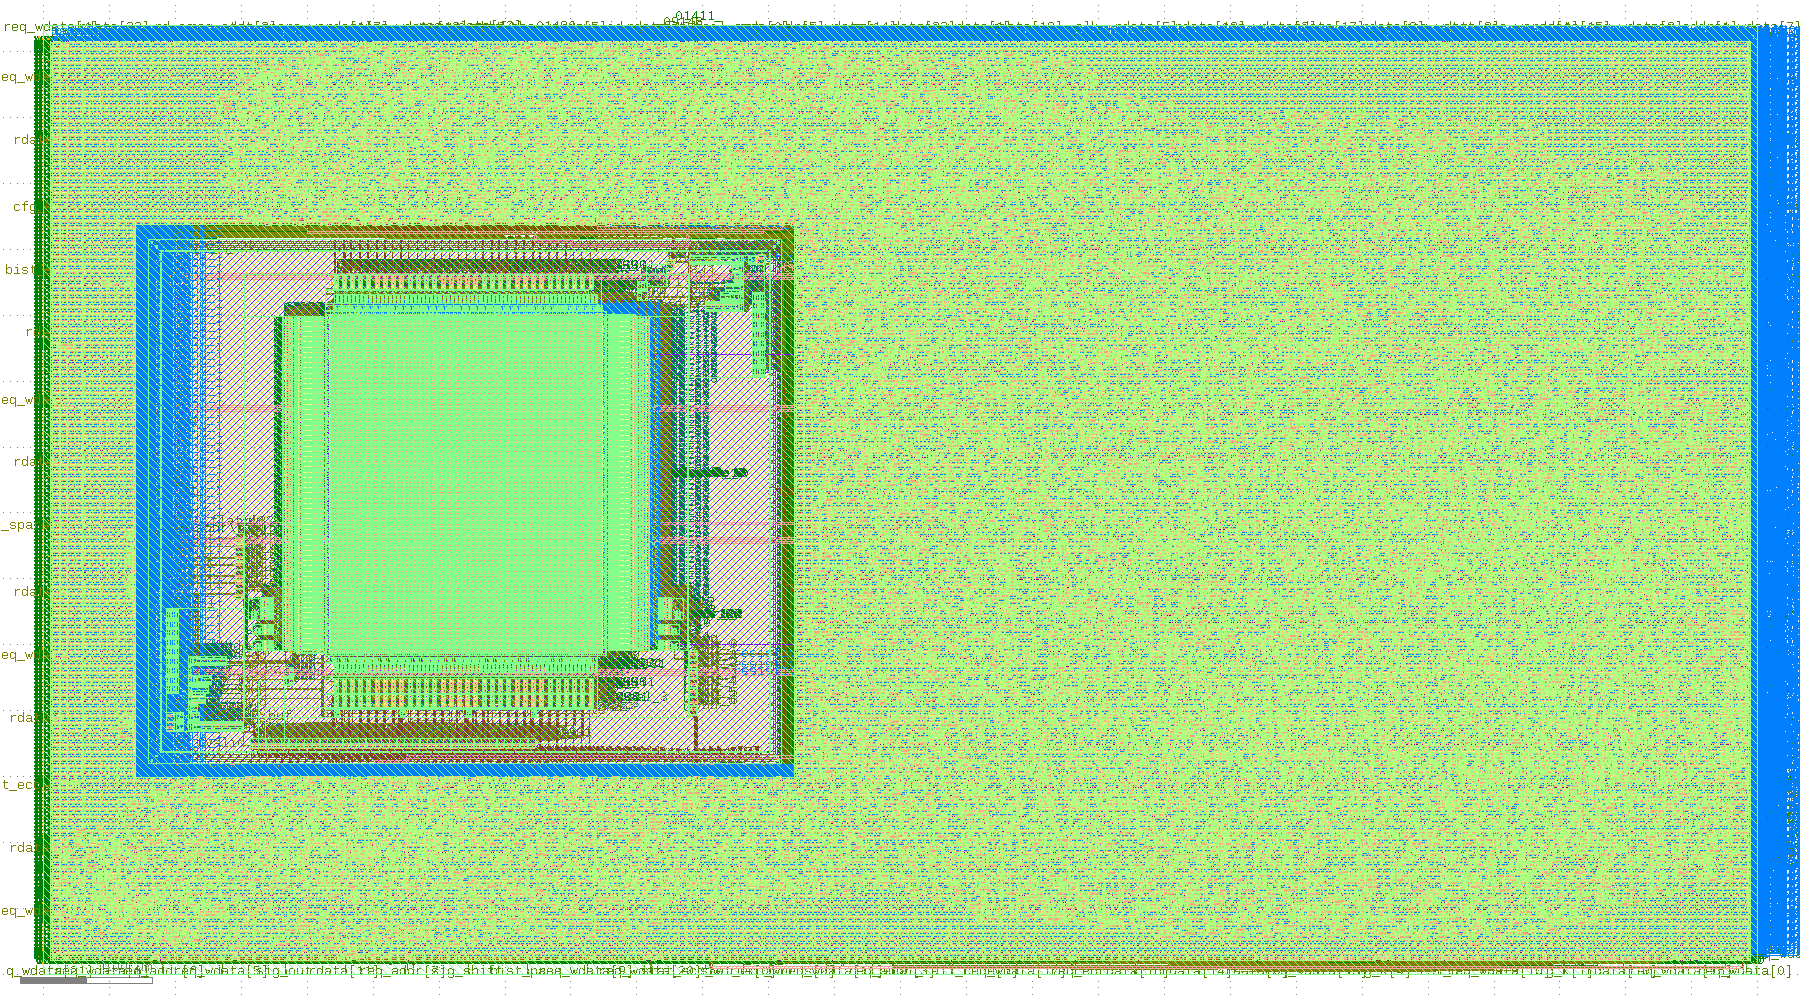
\includegraphics[width=\columnwidth]{../results/asic/try15/layout.png}
\caption{Routed layout, $1.30\times0.72$\,mm. The macro is at the left.}
\label{fig:layout}
\end{figure}

The design was implemented with OpenLane 1.0.2 at a 40\,ns clock on a 0.936\,mm$^2$ die
(Fig.~\ref{fig:layout}). Table~\ref{tab:signoff} gives the status. The layout is not sign-off clean.
The slew violations lie on nets that receive antenna diodes after the last buffering step of the flow,
and raising the buffering margin far enough made the tool hang; antenna and slew traded against each
other across runs. The macro is treated as verified IP in LVS and in the design-rule check. Its
timing model has a single corner, so the clock mainly reflects the wrapper. The power figure of
27\,mW is a vectorless estimate that excludes the macro.

\begin{table}[t]
\caption{Sign-off status of the routed design}
\label{tab:signoff}
\centering
\begin{tabular}{@{}lr@{}}
\toprule
Check & Result \\
\midrule
Detailed-routing violations & 0 \\
LVS errors & 0 \\
Worst setup / hold slack over RC corners & 1.95 / 0.10\,ns \\
Design-rule check of the final GDS, macro abstract & 0 \\
Antenna violations & 1 \\
Maximum-slew violations (worst 1.33 against 0.75\,ns) & 200 pins \\
Maximum-fanout violations (limit 10) & 1705 \\
\bottomrule
\end{tabular}
\end{table}

\section{Limitations}
There is no silicon. The memory is small, and the defect mixes and the soft-error rate are
assumptions, which is why results are given per mix. Spares are fault-free in the Monte Carlo study,
although the hardware handles faulty spare columns. Multi-bit upsets are not modelled. The baselines
that use ECC first were built from published descriptions. The proofs have not been reviewed by a
second person.

\section{Conclusion}
Treating ECC as a budgeted repair resource and steering spare columns per address partition lets a
small on-chip allocator stay exact and lets the designer cap the soft-error cost of repair. The
benefit depends on the defect mix: it is large for cell and cluster defects and absent for line
defects. The complete design, models and results are available at
\url{https://github.com/hieuminhvo250221-del/triad-bisr}.

\bibliographystyle{IEEEtran}
\bibliography{refs}
\end{document}
